\section{Comparison of FSL FIX and Standard Preprocessing}

The following section will present the results using both the standard preprocessing pipeline and FSL FIX pipeline. First, the signal of brain activation related to the 48$^\circ$ stimulus, achieved from using both methods is presented. Secondly, will the difference in amount if activation achieved by using FSL FIX compared to standard preprocessing be presented. \\
As mentioned in \secref{stats} a within heat run, within participant and within group analysis, were run on the cleaned fMRI data. \Figref{fig:res:stdpos} and \figref{fig:res:stdneg} shows the Z-score and localization of the activation achieved using the standard preprocessing pipeline.  


\begin{figure}[H]                 
	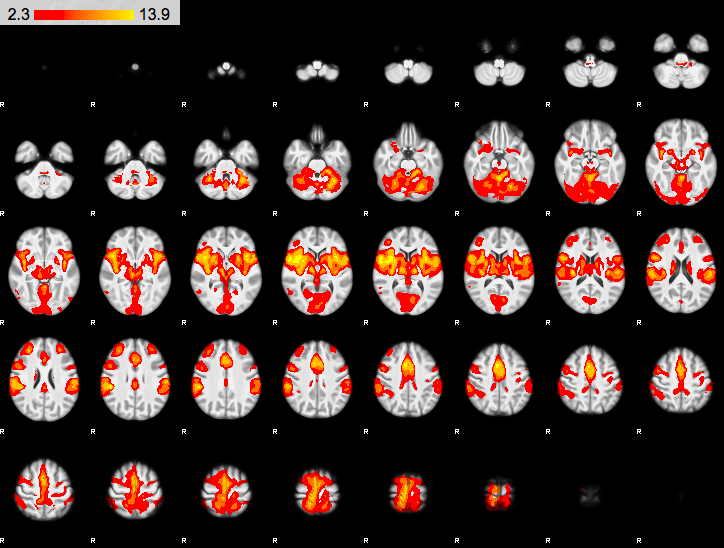
\includegraphics[width=.65\textwidth]{figures/Results/STD_pos}  
	\caption{Results of the achieved positive brain activation. The activation is mainly localized in the regions of the insular cortex, basal ganglia, anterior cingulate cortex, and sensorimotor cortex.}
	\label{fig:res:stdpos} 
\end{figure}

\begin{figure}[H]                 
	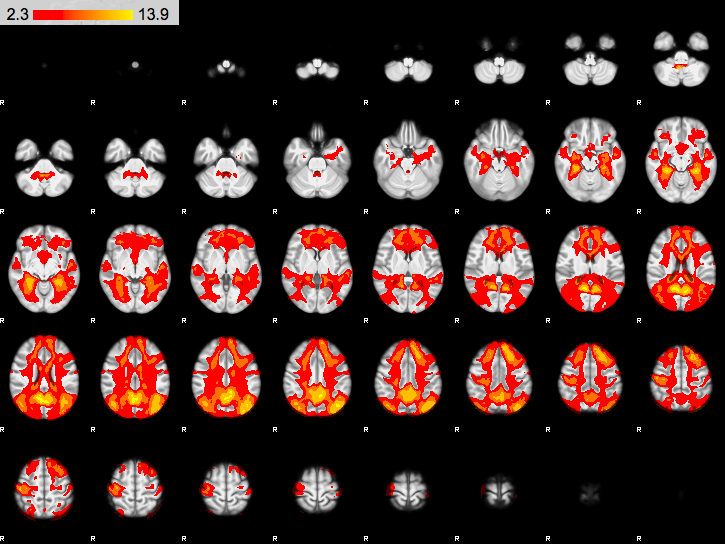
\includegraphics[width=.65\textwidth]{figures/Results/STD_neg}  
	\caption{Results of the achieved negative brain activation. The negative activation is mainly localized in the white matter and the default mode network (prefontal cortex and posterior cingulate cortex).}
	\label{fig:res:stdneg} 
\end{figure}

The localization of regions which are activated during the noxious heat stimuli are primarily those anticipated as presented in \secref{sec:pain}. The main activation is localized in the regions of the insular cortex, basal ganglia, anterior cingulate cortex, and sensorimotor cortex. The Z-score of the map has a range 2.3 to 13.9. \\
\Figref{fig:res:FIXpos} and \figref{fig:res:FIXneg} shows the intensity and localization of the activation achieved using the FSL FIX preprocessing pipeline. 

\begin{figure}[H]                 
	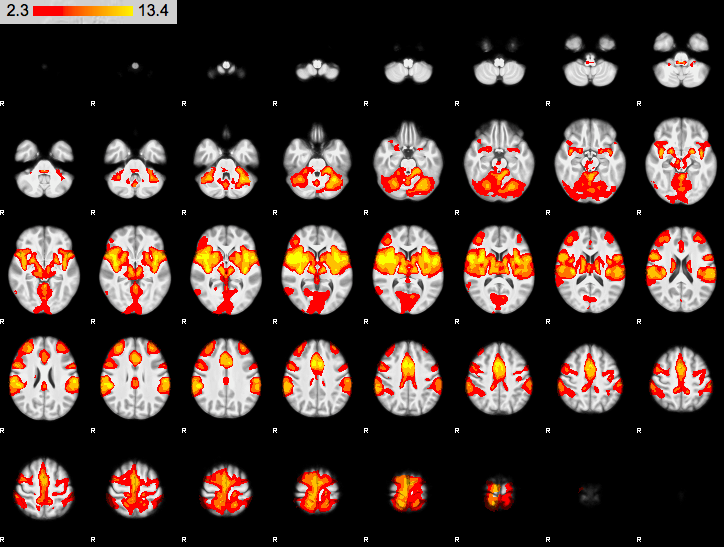
\includegraphics[width=.65\textwidth]{figures/Results/FIX_pos}  
	\caption{Results of the achieved positive brain activation. The activation is mainly localized in the regions of the insular cortex, basal ganglia, anterior cingulate cortex, and sensorimotor cortex.}
	\label{fig:res:FIXpos} 
\end{figure}

\begin{figure}[H]                 
	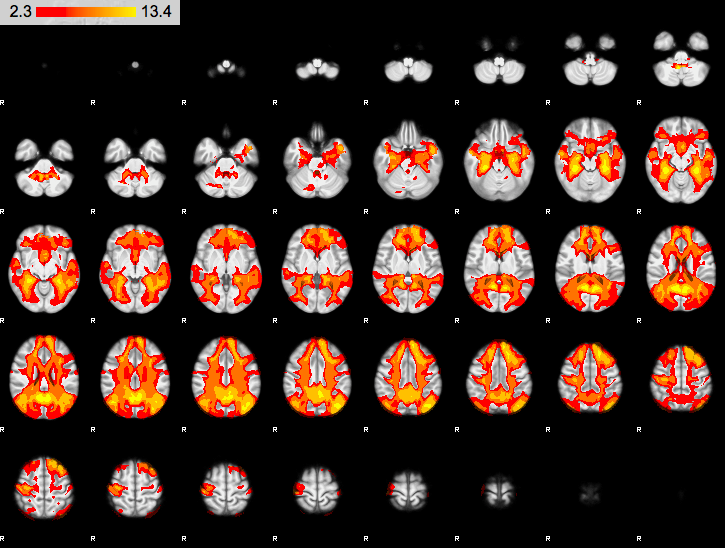
\includegraphics[width=.65\textwidth]{figures/Results/FIX_neg}  
	\caption{Results of the achieved negative brain activation. The negative activation is mainly localized in the white matter and the default mode network.}
	\label{fig:res:FIXneg} 
\end{figure}

The localization and intensity of the activation found by using FIX is very similar to the one seen using standard preprocessing. The Z-score range is though a bit less as it ranges from 2.3 to 13.4.\\
From the results of using the standard preprocessing pipeline and FSL FIX pipeline the results seem fairly identical. In both cases the same localization of activation were found both in the positive and negative activation map.   
To get statistical measure of the difference in localization and intensity between the two preprocessing methods a comparison was made. The results of this comparison is seen in \figref{fig:res:diff_pos} and \figref{fig:res:diff_neg}. 

\begin{figure}[H]                 
	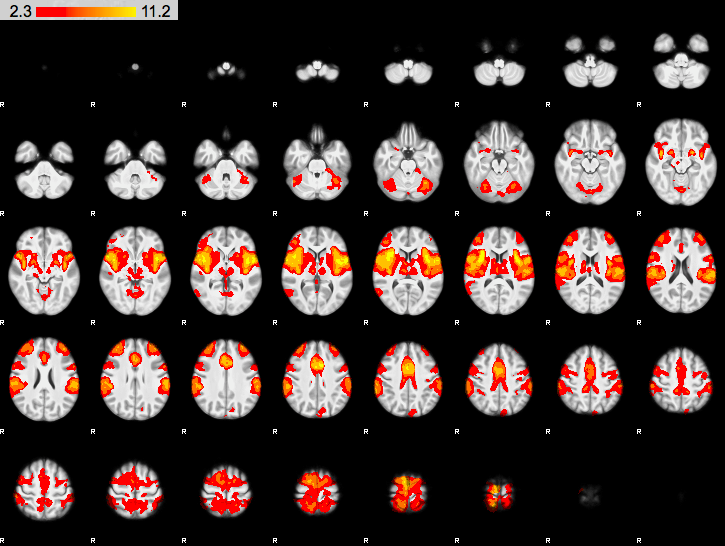
\includegraphics[width=.65\textwidth]{figures/Results/diff_pos}  
	\caption{Results from the comparison of the two preprocessing methods for noise removal. The activation seen is the activation gained with using FIX. Increased signal is mainly seen in the insular cortex, anterior cingulate cortex and basal ganglia.}
	\label{fig:res:diff_pos} 
\end{figure}

\begin{figure}[H]                 
	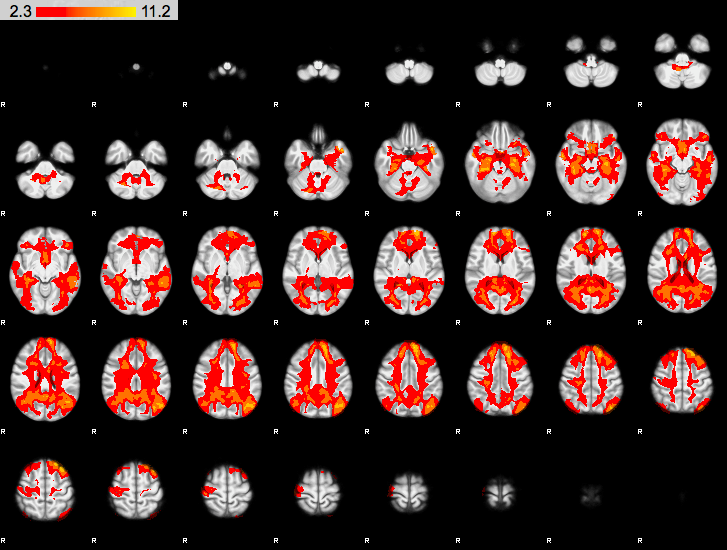
\includegraphics[width=.65\textwidth]{figures/Results/diff_neg}  
	\caption{Results from the comparison of the two preprocessing methods for noise removal. The activation seen in the image is the amount of activation which have been removed by using FIX compared to standard preprocessing. Areas where activation have been removed are white matter and default mode network.}
	\label{fig:res:diff_neg} 
\end{figure}

To summarize the results of using FSL FIX after standard preprocessing compared to solely using standard preprocessing, FSL FIX does achieve a higher signal-to-noise ratio. This is especially clear in \figref{fig:res:diff_pos} where a relatively high Z-score was achieved. 
